\documentclass[11pt,a4paper]{article}

% Underscores must survive pdftotext -- this PDF is converted for a reader and
% a search index, so a lost underscore is a lost identifier. OT1 draws \_ as a
% RULE, not a glyph, so \pdfgentounicode cannot map it. T1 makes _ a real
% character. Verified by extraction in build.sh; do NOT add microtype.
\usepackage[T1]{fontenc}
\usepackage{lmodern}
\input{glyphtounicode}
\pdfgentounicode=1

\usepackage[margin=1in]{geometry}
\usepackage{booktabs}
\usepackage{array}
\usepackage{amsmath}
\usepackage{amssymb}
\usepackage{stmaryrd}   % \llbracket, \rrbracket for semantic brackets
\usepackage{tikz}       % Figure 1 (state-space folding)
\usepackage{hyperref}
\hypersetup{colorlinks=true,linkcolor=black,urlcolor=black,citecolor=black}

\newcommand{\paperversion}{16}

\title{Folding: Recovering Precision in Interval-Based Static Analysis}
\author{Adi Oltean \\ \texttt{adi@starcloud.com}\thanks{This document was prepared with
AI assistance: drafting, literature search, and citation verification were AI-assisted,
under human direction and review.}}
\date{2026-08-20 \quad (v\paperversion)}

\begin{document}
\maketitle

\begin{abstract}
\noindent
A sound static analysis built on a non-relational interval domain --- optionally
augmented by a small set of relational side tables --- loses precision wherever a
program's reachable states are scattered. \emph{Folding} is a technique for recovering
that precision without enriching the domain: a catalogue of recognizers matches loop,
layout, encoding, state and relational shapes, and each match supplies the analysis with
a fact that is valid at a specific program point. This note gives the intuition behind
folding, describes the mechanism and the soundness obligation it carries, presents the
full pattern catalogue, shows that folds landing on a \emph{contiguous} range are exact
--- and therefore generate concrete counterexamples as well as safety proofs --- measures
how much precision is recovered, sketches how folds might be proposed automatically
under the same admission discipline, and situates the technique in the
abstract-interpretation literature.
\end{abstract}

\section{Motivation}\footnote{\textbf{Artifact.} Source, evaluation and proofs are in
the public repository \url{https://github.com/adi-oltean/folding-paper}; reproduce with
\texttt{python3 eval/run.py --check}. The theorems of \S\ref{sec:exactness} are
discharged by exhaustive enumeration at finite widths in \texttt{eval/proof/} and
mechanized in Lean in \texttt{proof-lean/} (sorry-free, no external dependencies).
Coverage is deliberately uneven by design --- most theorems are Lean-proved for all
parameters, some rest on the finite-width enumeration instead --- with the per-theorem
ledger in \texttt{proof-lean/README.md}.}
An interval domain cannot represent a stride. In

\begin{verbatim}
    for (int i = 0; i < n; i += 4) { ... a[i] ... }
\end{verbatim}

\noindent
the analysis learns $i \in [0, n)$ and loses $i \equiv 0 \pmod 4$. The usual remedies
enrich the domain --- strided intervals~\cite{balakrishnan2010}, congruence
domains~\cite{granger1989}, trace partitioning~\cite{rival2007} --- and each enrichment
adds cost to every join, meet and widening in the analysis, including on code containing
none of the patterns it was introduced for.

Folding takes the alternative route: for a set of recognizable shapes, derive the missing
fact from the program and supply it to the unmodified domain at the point where it holds.

\subsection{Intuition: folding the state space}
\label{sec:intuition}

The name is the intuition. The loop above reaches a \emph{scattered} set of states ---
$i \in \{0, 4, 8, \dots\}$, stretched across $[0, n)$ --- and between the reachable points
lie \emph{dead bands}: values the program never takes, which a convex approximation must
nevertheless include. Folding eliminates the dead bands by geometrically folding the state
space --- pleating a tape measure so that only the marked points remain on the face and
the blank spans between them are taken up into the folds. Concretely, divide by the
stride: the scattered points $\{0,4,8,\dots\}$ land on the contiguous segment
$\{0,1,2,\dots\}$, in order and without collision. Nothing is lost --- the set is re-described in coordinates where it is
compact, and in those coordinates a convex domain represents it \emph{exactly}.
Figure~\ref{fig:fold} shows the fold.

\begin{figure}[t]
\centering
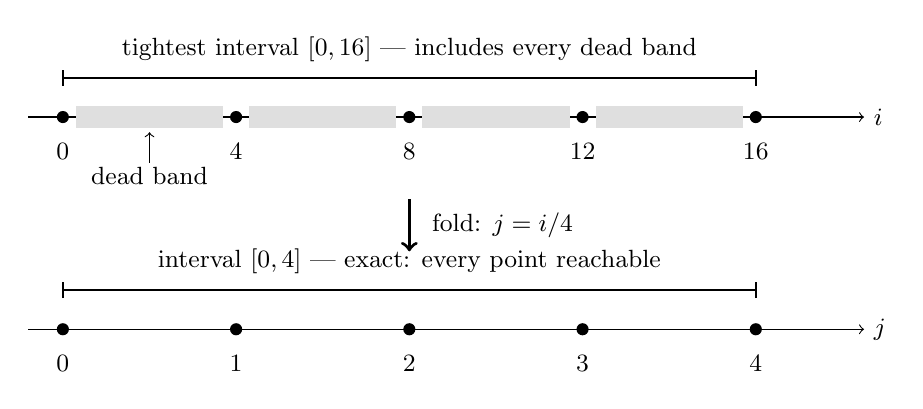
\begin{tikzpicture}[scale=0.55]
% ---- unfolded coordinate ----
\draw[->] (-0.8,0) -- (18.5,0) node[right] {\small $i$};
\foreach \x in {0,4,8,12} {
  \fill[gray!25] (\x+0.3,-0.26) rectangle (\x+3.7,0.26);
}
\foreach \x in {0,4,8,12,16} \fill (\x,0) circle (0.14);
\foreach \x/\l in {0/0,4/4,8/8,12/12,16/16} \node[below=6pt] at (\x,0) {\small $\l$};
\draw[thick] (0,0.9) -- (16,0.9);
\draw[thick] (0,0.72) -- (0,1.08);
\draw[thick] (16,0.72) -- (16,1.08);
\node[above] at (8,1.05) {\small tightest interval $[0,16]$ --- includes every dead band};
\node at (2,-1.35) {\small dead band};
\draw[->] (2,-1.05) -- (2,-0.35);
% ---- the fold ----
\draw[->, very thick] (8,-1.9) -- (8,-3.1);
\node[right] at (8.3,-2.5) {\small fold: $j = i/4$};
% ---- folded coordinate ----
\begin{scope}[yshift=-4.9cm]
\draw[->] (-0.8,0) -- (18.5,0) node[right] {\small $j$};
\foreach \x/\l in {0/0,4/1,8/2,12/3,16/4} {\fill (\x,0) circle (0.14);
  \node[below=6pt] at (\x,0) {\small $\l$};}
\draw[thick] (0,0.9) -- (16,0.9);
\draw[thick] (0,0.72) -- (0,1.08);
\draw[thick] (16,0.72) -- (16,1.08);
\node[above] at (8,1.05) {\small interval $[0,4]$ --- exact: every point reachable};
\end{scope}
\end{tikzpicture}
\caption{Folding the state space of \texttt{for (i = 0; i < 20; i += 4)}. Above: the
reachable values of $i$ are scattered, and the tightest convex approximation must include
the dead bands between them. Below: after the change of variables $j = i/4$, the reachable
set is contiguous and the interval represents it exactly; $i$ is recovered as $4j$ where
used.}
\label{fig:fold}
\end{figure}

To achieve this, folding conceptually changes the underlying code: it is a change of
variables. The loop is re-expressed to walk the folded coordinate --- $j = i/4$, stepping
by one --- so that the state space the analysis must represent is the compact one, while
the original $i$ is recovered as $4j$ exactly where it is used. The program's semantics is
untouched; what folds is the \emph{shape of its state space} as the abstract domain sees
it. The change of variables can be realized either by rewriting the code or by supplying
the folded facts directly to the analysis; folding takes the second route, described next.

\section{Mechanism}
\label{sec:mechanism}

Folding runs in two stages.

\paragraph{Detection.} Once per function, before the fixpoint, a single pass over the CFG
nodes matches program shapes against the pattern catalogue of \S\ref{sec:patterns}. A
match produces a metadata record. A shape the catalogue does not match contributes no
extra fact and is analysed exactly as it would be without folding --- non-recognition is
conservative, never an error and never a lost verdict.

\paragraph{Consumption.} During the fixpoint, at specific program points --- the
true-branch edge out of a loop header, back edges, and if/else merge points --- the
recorded facts are met into the abstract state, contributed as widening thresholds, or
written into relational side tables.

Folding performs no program transformation. There is no source-to-source rewriting, no
CFG mutation, and no fresh loop variable in the program text: detection reads the CFG
and returns metadata, and the CFG is never modified. Nor is
folding a separate pre-pass in the usual sense --- only detection precedes the fixpoint,
while consumption happens inside it, per edge, per iteration. Folds discovered within a
function serve that function directly; because the surrounding analysis is
interprocedural (bottom-up, summary-based), a fold fact is as summarizable as any other
analysis fact (\S\ref{sec:xproc}).

\subsection{The soundness obligation}
\label{sec:validity}

Because nothing is transformed, semantics preservation is not the relevant property. The
obligation is a validity condition on each injected fact:

\begin{quote}
For a fact $F$ injected at program point $p$: every concrete state reachable at $p$ must
satisfy $F$ --- equivalently, the set of states reachable at $p$ is contained in
$\gamma(F)$. Given that, replacing the abstract state $a$ at $p$ by $a \sqcap F$ removes
no reachable state, and the analysis remains an over-approximation.
\end{quote}

The direction of failure is worth being explicit about. Meeting a bound is subtractive: an
invalid fact does not merely cost precision, it removes reachable states from the
abstraction, which is the direction that produces unsound results rather than false
alarms. Each pattern therefore carries its own validity condition, and admission of a fact
(\S\ref{sec:certs}) is exactly the establishment of that condition: a shape whose
condition cannot be established supplies no fact.

\paragraph{Is this just \texttt{assume}?} The objection should be put at its strongest,
because the answer to it locates whatever is new here. Injecting a fact $F$ that is
invariant at $p$ is \emph{semantically identical} to analysing a program instrumented with
\texttt{assume($F$)} at $p$, whose instrumentation is a concrete no-op on reachable states
(stated formally in \S\ref{sec:assume-formal}); the injection primitive is not new, and neither are the individual
resemblances --- pattern 7 is the data-space analogue of trace partitioning, pattern 1's
closed form is a trip-count computation every compiler performs. So the content is not the
primitive but three things around it. First, \emph{where the cost falls}: a fact met at the
points it holds leaves join, meet and widening untouched, while representing the same
information in the domain pays at every abstract operation on every program, whether or not
the shape occurs. Second, \emph{who is allowed to propose}: under certificate admission
(\S\ref{sec:certs}) the proposer is outside the trusted base entirely, so facts may be
proposed by any heuristic whatever --- which is what a hand-written \texttt{assume} is
not, since it is trusted by virtue of being written. Third, \emph{what a fold can be
proved to buy}: a fold meeting the hypothesis of \S\ref{sec:exactness} is simultaneously a
sound over- and under-approximation, so it yields concrete counterexamples and not only
proofs. An \texttt{assume} is a place to put a fact; the catalogue, its validity
conditions, the admission architecture and the exactness result are what make supplying one
a technique.

\section{The pattern catalogue}
\label{sec:patterns}

Every pattern folds the state space along some axis of its \emph{generating map} ---
the function that produces the reachable states from the program's actual degrees of
freedom, whether that is a loop's iteration count, a layout function over an index, or an
encoding: \emph{time}
(the iterates of a loop), \emph{space} (the layout of data), \emph{value} (an arithmetic
or bit-level encoding), \emph{control} (the legal states of a state machine), or a
\emph{relation} between variables.

\begin{center}
\begin{tabular}{clp{7.0cm}}
\toprule
\# & Pattern (axis) & Fact supplied \\
\midrule
1 & Affine induction variable (time) & $i \le \mathit{actual\_max}$ (descending:
    $i \ge \mathit{actual\_min}$), plus widening thresholds \\
2 & While-$\ne$ induction variable (time) & $i \le N$, via divisibility of the distance
    to the limit \\
3 & Geometric induction variable (time) & $m = 2^t$: single set bit, bounded exponent \\
4 & Polynomial accumulator (time) & closed-form bound on a running sum \\
\midrule
5 & Struct field factoring (space) & element size for the bounds computation \\
6 & Stride-union convexification (space) & a field-index variable over a convexified
    offset set \\
7 & Residue partition (space) & per-phase facts on interleaved arrays \\
\midrule
8 & Bitfield decomposition (value) & known-bit masks (a \texttt{KnownBits} reduced
    product) \\
9 & Modular arithmetic (value) & quotient/remainder relationships \\
10 & Bit-slice range (value) & \texttt{(x >> k) \& m} $\in [0, m]$ \\
11 & Monotone mask accumulation (value) & a grows-only bit set under \texttt{|=} \\
12 & Two-sided clamp (value) & $v \in [\mathit{lo}, \mathit{hi}]$ after saturation \\
13 & Bijective encoding transport (value) & the exact image interval through a named
    bijection \\
\midrule
14 & Sparse-state rank (control) & $\mathit{state} \in S$ for a finite legal set \\
\midrule
15 & Conditional variable splitting (relation) & $x \le y$ in a relational side table \\
16 & Lockstep elimination (relation) & $p = \mathit{base} + s \cdot i$, folding a 2D
    line onto one variable \\
\midrule
17 & Conserved-pair cursor (relation) & $p - \mathit{base} + r = \mathit{const}$ for a
    cursor/remaining pair advanced by data-dependent amounts \\
18 & Lower-bounded variable stride (time) & trip bound $\lceil r_0 / s_{\min} \rceil$
    from a guard-established minimum decrement \\
19 & Modular difference band (relation $\times$ value) & $\mathit{in} - \mathit{out} \in
    [0, \mathit{size}]$ for free-running wrapping counters \\
20 & Sign-mask broadcast select (value) & $m \in \{0, 2^w{-}1\}$, and the select's range
    is the union of its two arms \\
21 & Add-with-carry recomposition (value) & $\mathit{cy} \in \{0,1\}$ through a limb
    chain \\
\bottomrule
\end{tabular}
\end{center}

The catalogue is open by construction --- the class of programs an analysis is complete
for is not recursively enumerable (\S\ref{sec:theory}), so new generating maps keep
producing new patterns. Every pattern follows the same recipe: a matched shape, a
supplied fact, a validity condition.

\subsection{Time folds (patterns 1--4)}

\paragraph{Pattern 1: the affine induction variable.} For
\texttt{for (i = c0; i $\bowtie$ L; i += s)} with $\bowtie\ \in \{<, \le, \ne\}$ and
$c_0, L, s$ literal constants, the last value $i$ takes on entry to the body (for a loop
whose body executes at least once; otherwise any fact at body entry is vacuous) is
computable exactly. For $<$ it is
$\mathit{actual\_max} = c_0 + s\lceil (L - c_0)/s \rceil - s$; for $\le$, the same
expression with $L$ replaced by $L+1$; for $\ne$, the guard is exact only when
$s \mid L - c_0$ \emph{and} $c_0 \le L$ --- divisibility alone is not enough, since it
holds equally for limits already passed (\texttt{i = 7; i != 5; i += 2} divides evenly
but never reaches $5$) --- in which case $\mathit{actual\_max} = L - s$; otherwise the
loop does not terminate at $L$ and the pattern declines the match.
Supplying $i \le \mathit{actual\_max}$ is strictly stronger than the header condition for
$<$ when $s > 1$ and $L - c_0 \not\equiv 1 \pmod{s}$, and for $\le$ under the same test on
$L+1$; otherwise the two coincide. For $\ne$ it is stronger unconditionally, the guard
having supplied no bound at all. Descending loops
(\texttt{i -= s}) are the mirror image, supplying $i \ge \mathit{actual\_min}$; symbolic
limits are handled by the certificate form of \S\ref{sec:symbolic}.
\emph{Validity condition:} $i$ is not modified in the body other than by the loop
increment, its address is not taken, and the increment does not wrap at the operand's
type ($\mathit{actual\_max} + s$ representable). The wrap clause is not pedantry:
unsigned wraparound is \emph{defined} behavior that silently re-enters the loop below the
bound, so excluding it is part of the obligation, not a given. The
payoff is bounds the plain interval domain cannot discharge --- \texttt{buf[i+1]} with
$\mathrm{len}(\mathtt{buf}) = 20$ under \texttt{i += 2} --- with corresponding
out-of-bounds cases still reported as failures.

\paragraph{Pattern 2: the while-$\ne$ induction variable.} The same fold for loops
guarded by disequality --- \texttt{while (i != N) i++;}. The guard alone bounds nothing
(an interval cannot subtract a point from its interior); the fold supplies $i \le N$,
valid because the stride divides the distance from the initial value to the limit, so the
iterates cannot step over $N$. \emph{Validity condition:} a single increment site, no
other writes, no address-taking, divisibility of $N - c_0$ by the stride, and
$c_0 \le N$ --- the iterates must approach the limit from below, or the fact fails at the
first body entry.

\paragraph{Pattern 3: the geometric induction variable.} Loops that scale rather than
step: \texttt{for (m = 1; m; m <<= 1)}, doubling searches, halving reductions --- bit
iteration, binary search, CRC and mantissa loops. The reachable set $\{1, 2, 4, \dots\}$
has geometrically growing dead bands; the fold is $t = \log_2 m$, under which it is
$\{0, 1, \dots, w{-}1\}$, contiguous. Facts supplied: $m$ has exactly one set bit, and
its exponent lies in a bounded range --- known-bits facts, carried by the same reduced
product as pattern 8. \emph{Validity condition:} $m$ is modified only by the one shift or
multiply, and the operand is \emph{unsigned} --- for a signed operand the shift into the
sign position is undefined (C11 \S6.5.7) before the bit could ever leave the word. For
loops that terminate by shifting the bit out, the termination argument is a width fact at
the operand's \emph{declared} type: the shift computes at the promoted width, but the
assignment truncates back, so a \texttt{uint8\_t} loop terminates after eight iterations,
not thirty-one.

\paragraph{Pattern 4: the polynomial accumulator.} A running sum of an induction
variable --- \texttt{s += i} --- has a closed form polynomial in the trip count
($s = t(t{-}1)/2$ for the triangular sum), so the fact is a closed-form bound on
\texttt{s}, per iteration or at exit; such bounds are what overflow proofs about
accumulated quantities need. \emph{Validity condition:} the accumulator is written only
by the recognized update, and the bound is evaluated at the folded trip count.

\subsection{Space folds (patterns 5--7)}

\paragraph{Pattern 5: struct field factoring.} An access \texttt{a[i].f} is factored
into element index, element size and field offset, and the element size is supplied to
the bounds computation so the index is checked against an element count rather than a
byte extent. \emph{Validity condition:} the accessed object's declared element type
matches the factored size.

\paragraph{Pattern 6: stride-union convexification.}
\label{sec:convex}
When a loop reads several fields of a struct array, the set of byte offsets touched is a
union of arithmetic progressions, and so non-convex; an interval must take the convex
hull, which covers the padding between fields --- the dead bands of the address space.
Dividing the offsets by the gcd of their differences maps, for example, $\{0,4,8\}$ to
$\{0,1,2\}$, which is convex and exactly representable, and the address is re-expressed
against a fresh field index. For equally spaced offsets the construction composes across
nesting levels: a non-convex set in one-dimensional address space becomes a box in a
higher-dimensional index space, exactly representable by independent intervals. Unequally
spaced offsets fold to a smaller but still non-convex set --- $\{0,4,6\}$ divided by its
gcd is $\{0,2,3\}$ --- where the fold shrinks the dead bands without eliminating them. \emph{Validity condition:}
the offsets and stride are those of the declared layout, and every access in the folded
region goes through the recognized index expressions.

\paragraph{Pattern 7: residue partition.} Interleaved data --- \texttt{buf[2i]} real,
\texttt{buf[2i+1]} imaginary --- is a union of residue classes. Where convexification
merges the classes into one folded range, the residue partition keeps them apart and
supplies a \emph{per-phase} fact for each (the even indices hold one kind of value, the
odd another); it is the data-space analogue of trace partitioning~\cite{rival2007}.
\emph{Validity condition:} every access to the region is through an index expression
with a recognized residue.

\subsection{Value folds (patterns 8--13)}

Value folds matter because much real C shapes \emph{values}, not indices. In a shape
census across twelve public C codebases (\S\ref{sec:eval}), mask accumulation and
bit-slice extraction are the most frequent foldable shapes; their weight is strongly
domain-dependent --- protocol-codec and cryptographic code rank highest (the codec at
$5.75\times$ against \texttt{for} loops), while query engines, libc internals and
protocol control flow fall well below.

\paragraph{Patterns 8--9: bitfields and modular arithmetic.} Bitfield packing and
\texttt{\%}/\texttt{/} pairs are encodings whose images are exactly representable by
known-bit masks (a \texttt{KnownBits} reduced product alongside the intervals) and by
quotient/remainder relationships. \emph{Validity conditions:} the declared field widths,
and the sign convention of C's truncating division.

\paragraph{Patterns 10--12: slices, masks and clamps.} Three interval-expressible facts:
a bit-slice \texttt{(x >> k) \& m} lies in $[0, m]$ for any operand and non-negative
mask; a flag word written only by \texttt{|=} grows monotonically within the set of bits
ever supplied; a value passed through a two-sided clamp lies in
$[\mathit{lo}, \mathit{hi}]$ at every subsequent use the clamp dominates.
\emph{Validity conditions:} respectively the expression shape alone; all writes are
recognized accumulations; the clamp dominates the uses with no intervening reassignment
of the clamped variable.

\paragraph{Pattern 13: bijective encoding transport.} Wire formats fold values by
design: ZigZag interleaves signs ($0, -1, 1, -2 \mapsto 0, 1, 2, 3$) precisely to
eliminate the dead band that sign-extension creates in varint
space\footnote{The mechanism is documented in Protocol Buffers' own encoding
specification (\url{https://protobuf.dev/programming-guides/encoding/}): without the
interleaving, a small negative integer sign-extends to a maximal-width varint.}; byte swaps permute
known bits; bit-reversal permutes an index range onto itself. For a bijection $g$ drawn
from a fixed, named library, the fold transports intervals \emph{exactly}: if
$x \in [-2^k, 2^k)$ then $\mathrm{zigzag}(x) \in [0, 2^{k+1})$, in both directions, the
image computed by a once-per-bijection lemma. \emph{Validity condition:} the expression
matches the bijection's canonical form at the operand's promoted width.

\subsection{Control folds (pattern 14)}

\paragraph{Pattern 14: sparse-state rank.} State machines over sparse or one-hot codes
--- $\mathit{state} \in \{\mathtt{0x01}, \mathtt{0x04}, \mathtt{0x10}\}$ --- scatter a
three-element legal set across an interval that is mostly dead band. Rank-indexing the
legal set folds it to $\{0, 1, 2\}$; the fact is $\mathit{state} \in S$, refined through
switch and comparison edges. \emph{Validity condition:} every assignment to the state
variable --- its initialization included --- is a member of $S$, and its address is not
taken: a closure condition over the variable's writes, carried across calls by the
summary form of \S\ref{sec:xproc}.

\subsection{Relation folds (patterns 15--16)}

\paragraph{Pattern 15: conditional variable splitting.} When both branches of a
conditional assign the same variable values with a known order, the merge point carries
the ordering fact $x \le y$ in a relational side table instead of losing it in the join.
\emph{Validity condition:} both branches are recognized single assignments.

\paragraph{Pattern 16: lockstep elimination.} Two variables advancing together ---
\texttt{p++} with \texttt{i++}, so $p = \mathit{base} + s \cdot i$ --- reach only a line
inside their product box; everything off the line is dead band. The fold eliminates one
variable by the affine relation, tracking $i$ and recovering $p$ at its uses.
\emph{Validity condition:} both variables are updated in the same iterations with the
recognized strides, and neither is modified elsewhere in the loop.

\subsection{Patterns from real code (17--21)}
\label{sec:corpus-patterns}

The first sixteen rows were derived from the shapes a domain loses precision on. The last
five were derived the other way round --- by reading kernel, cryptographic, database,
libc and network C and asking what defeats an interval domain there. They are stated here
with their validity conditions; unlike rows 1--16 they carry no evaluation instance in
\S\ref{sec:eval}, and are offered as catalogue entries rather than measured results.

\paragraph{Pattern 17: conserved-pair cursor.} A cursor and a remaining-length counter
advanced by \emph{equal and opposite, data-dependent} amounts --- the skeleton of every
length-prefixed record parser (\texttt{p += len; rem -= len}). The conserved quantity
$p - \mathit{base} + r$ is invariant, so any guard on $r$ transfers to a bound on $p$.
Without it a non-relational domain must widen the cursor as soon as the advances become
data-dependent, losing the bound the parser's own guards establish. \emph{Validity
condition:} every update to either variable inside the region is paired, in the same
basic block, with an update to the other by the same amount and opposite sign, that
amount evaluated once; neither variable's address is taken; and the cursor advance does
not wrap at the operand's type. Generalizes pattern 16 to non-constant strides.

\paragraph{Pattern 18: lower-bounded variable stride.} A loop whose decrement is not
constant but is bounded below by a guard --- an options walker that consumes at least two
bytes per iteration. The fact is a trip bound $\lceil r_0 / s_{\min} \rceil$, and with it
a bound on the cursor. \emph{Validity condition:} every path from header to back edge
decreases the remaining counter by an amount that path's guards bound below by
$s_{\min} \ge 1$; the counter is modified nowhere else; paths that do not decrease it
exit. Generalizes patterns 1--2 away from literal strides.

\paragraph{Pattern 19: modular difference band.} Two unsigned counters that only grow and
wrap freely at $2^w$, consumed only through their difference --- the ring-buffer idiom,
and the sequence-number comparison idiom. This is the one pattern where an interval domain
holds \emph{nothing} after the first wrap, while the difference coordinate stays exact:
$\mathit{in} - \mathit{out} \in [0, \mathit{size}]$ is an invariant even though neither
counter is bounded at all. \emph{Validity condition:} the counters start equal or at a
known constant difference; every increment is guarded so the difference cannot exceed
$\mathit{size} < 2^w$; every increment to the trailing counter is guarded by the current
difference; both are written only at recognized sites and their addresses are not taken;
all reads go through the difference or a masked projection of it. Under these, the
difference computed in $w$-bit unsigned arithmetic equals the true occupancy despite
either counter wrapping --- that wrap is defined behaviour and is the design.

\paragraph{Pattern 20: sign-mask broadcast select.} A comparison materialized as an
all-ones or all-zeros word and consumed by \texttt{AND}/\texttt{OR}/\texttt{XOR} instead
of a branch --- the constant-time cryptographic idiom. The fact is that the mask is
two-valued, $m \in \{0, 2^w{-}1\}$, from which a select's result range is the union of its
two arms rather than the hull of everything. \emph{Validity condition:} the mask is
defined by a recognized broadcast form --- $0 - b$ with $b \in \{0,1\}$ established,
$(x \gg (w{-}1))$ followed by $0-{}$ or ${}-1$, or $\sim$ of an existing mask --- at the
operand's promoted width; and between definition and consumption it flows only through
$\sim$, \texttt{\&}, \texttt{|}, \texttt{\textasciicircum} with other masks, or is consumed by a
recognized select or swap form (a masked XOR-swap of two variables is the same fact
applied twice), with no arithmetic other than the defining subtraction touching it. Optimization barriers are the live difficulty rather than a corner case: the
constant-time idiom routes masks through inline-asm or \texttt{volatile} identity
functions precisely to defeat value tracking, and they defeat this recognizer too. Such a
barrier must either be modelled as the identity --- a trusted fact, admitted per idiom ---
or the match declined.

\paragraph{Pattern 21: add-with-carry recomposition.} In multi-limb arithmetic, a carry
recovered by comparing a limb sum against one of \emph{its own} operands
(\texttt{c = (a+b) < a} detects overflow of that same addition). The fact is
$\mathit{cy} \in \{0,1\}$ threaded through the chain, which bounds every limb.
\emph{Validity condition:} the statement sequence matches the recognized
add-with-carry form --- each comparison tests the sum of an addition against an operand
of that same addition, at most two such additions per limb, with their carries combined
by \texttt{+} or \texttt{|}, all at the promoted width, and the carry entering the
sequence in $\{0,1\}$ --- the base case $\mathit{cy} = 0$ at loop entry, the induction step
being the lemma itself. This row is deliberately narrow, and earns its place only when a
limb combines \emph{two} such carries (the double-comparison case), where the needed fact
is a two-comparison correlation no non-relational domain sees. Three adjacent shapes do
not need it: a carry recovered by a
\emph{single} comparison, and a carry propagated through a mask-\texttt{AND}, are already
in $\{0,1\}$ under any reasonable comparison and bitwise transfer, so a plain interval
domain gets them free; the widening-multiply spelling, where the carry is extracted by a
shift, is covered by pattern 10.

\section{Admitting facts}
\label{sec:certs}

A fold fact is admitted into the analysis on one of two strengths. The first is
\emph{guarded detection}: the detector's guards establish the validity condition, and a
shape that cannot be guarded is not matched. The second fits a producer/verifier
architecture: the producer proposes facts by \emph{any} heuristic, and each fact enters
the analysis only through a per-instance certificate that an independent checker
verifies; a fact that cannot be certified becomes an explicit hypothesis rather than a
silent trust. Under certificate admission each fact kind splits into an \emph{arithmetic
half} --- the closed form of a recurrence, proved once per kind by induction and
thereafter merely evaluated --- and a \emph{shape half}, per-instance conformance
conditions on the program: the validity conditions of \S\ref{sec:validity}, carried as
certificate obligations rather than detector guards. Certificate admission removes the
detector from the trusted base entirely, which is what permits arbitrarily aggressive
proposers.

The compiler literature ships this shape with the polarity
reversed.\footnote{\texttt{gcc/tree-ssa-loop-niter.cc}
(\texttt{number\_of\_iterations\_exit}); \texttt{llvm/include/llvm/Analysis/}
\texttt{ScalarEvolution.h} (\texttt{PredicatedScalarEvolution}). Implementation
behaviour, cited to source rather than to a publication --- neither analysis has a
primary paper.} GCC's loop-iteration analysis returns counts together with explicit
\texttt{assumptions} predicates, and LLVM's predicated scalar evolution returns
recurrences \emph{under} predicates the client must discharge. A compiler may assume what it cannot prove, because the language standard
blames the program; a sound analyzer may not --- but inverting each assumption into a
checked obligation is exactly what a certificate is for.

\subsection{Symbolic bounds}
\label{sec:symbolic}

Bounds need not be literal. For \texttt{for (i = c0; i < L; i += s)} with
\emph{symbolic} $L$, the producer emits the claimed last body-entry value $m$ together
with a divisibility witness $q$, and the checker verifies four linear facts:
\[
m - c_0 = s\,q \;\wedge\; q \ge 0, \qquad m < L, \qquad m + s \ge L, \qquad
m + s \le M_\tau,
\]
where $M_\tau$ is the maximum of the operand's type. The first pair places $m$ on the
loop's residue, the next two bracket it against the guard, and the last excludes
wraparound --- for unsigned operands overflow is \emph{defined} behavior that re-enters
the loop below the bound, so the no-wrap assumption a compiler is entitled to make
returns here as a checked obligation. From these facts, $i \le m$ at body entry is
inductive, the induction step leaning on the shape half of the obligation: the
single-increment condition is what keeps $i$ on the residue $c_0 \bmod s$. The $\le$
guard replaces the bracket with $m \le L$ and $m + s > L$; the $\ne$ guard with
$m + s = L$. The checker performs no division and no trip-count computation, and never
reconstructs how the producer found $m$; the facts pin $m$ uniquely, so a wrong $m$ ---
too large or too small --- is rejected by the checker itself, and soundness never depends
on how the producer computed it. Scalar-evolution-style closed forms
(chains of recurrences~\cite{vanengelen2001}) generalize the same move to a catalogue
over \emph{semantic} shapes rather than syntactic spellings, and monotonicity-only facts
--- direction without a closed form --- are a still-cheaper entry point.

\subsection{Cross-procedure folds}
\label{sec:xproc}

The analysis is interprocedural, and folds cross call boundaries in two natural forms.
First, a callee summary can \emph{expose} the structure a caller's detector needs ---
e.g.\ that a callee consumes \texttt{(buf, len)} with a stride-$s$ access pattern --- so
the caller can discover a folding whose shape spans the call boundary. Second, a fold
fact established in a callee (a bound on a returned index, a monotonicity fact about an
updated field) can be \emph{transported} through the summary like any other
postcondition, with its validity condition re-expressed at the call site. In the
certificate framing of \S\ref{sec:certs}, both reduce to the same obligation shape: the
summary carries the fact plus the hypotheses under which it holds, and the caller's
certificate discharges those hypotheses at each call site.

\section{Exactness, and what it buys}
\label{sec:exactness}

Folding's validity condition (\S\ref{sec:validity}) asks only that an injected fact hold
of every reachable state --- an \emph{over}-approximation property, which is what safety
proofs need. Some folds satisfy something strictly stronger, and it has a consequence
worth isolating.

\begin{quote}
\textbf{Theorem (exactness).} Let $g$ be a fold that maps the reachable set $R$
\emph{bijectively onto a contiguous integer range}, write $R_g = g(R)$ for that folded
reachable set and $a_g$ for its tightest interval abstraction. Then the folded reachable
set is exactly an interval: $\gamma(a_g) = R_g$, so the abstraction is simultaneously a sound
\emph{over}-approximation and a sound \emph{under}-approximation.
\end{quote}

\noindent
The proof is immediate once the hypothesis is stated that way --- a contiguous range
equals its own interval hull, so no dead band survives --- and the work is in discharging
the hypothesis per fold: the affine induction variable $g(i) = (i-c_0)/s$ carries the
progression $\{c_0, c_0+s, \dots\}$ onto $\{0,\dots,m-1\}$; ZigZag carries the
\emph{full} symmetric range $[-2^k, 2^k)$ onto $[0, 2^{k+1})$; lockstep elimination
projects a line in the product space onto $\{0,\dots,n-1\}$.

Bijectivity alone is \emph{not} sufficient, and the distinction is not academic:
$g(i) = 2i$ is a bijection onto a stride-2 set, which is exactly the dead-band situation
folding exists to remove. The catalogue's own ZigZag instance makes the point --- applied
to the non-negative half $[0, 2^k)$ rather than the full symmetric range, it lands on the
even values only, and is measurably not exact ($\mathrm{DBF} = 1/2$ in
\S\ref{sec:eval}). Contiguity of the image, not invertibility, is what the theorem
needs.

The under-approximation half is the interesting one, because over-approximate analyses
cannot ordinarily supply it. If $\gamma(a_g) \subseteq R_g$, then every value the
abstraction admits is genuinely reachable --- so a failed check in folded coordinates is
not a \emph{maybe}. Applying $g^{-1}$ to the failing value yields a concrete, reachable
input that violates the check:

\begin{quote}
\textbf{Corollary (self-witnessing).} For a fold satisfying the theorem's hypothesis ---
bijective \emph{onto a contiguous range} --- the inverse of the fold is a counterexample
generator: an alarm in the folded coordinate back-substitutes to a concrete witness, with
no symbolic-execution or bounded-model-checking engine. Invertibility alone does not
suffice, for the same reason it does not suffice for exactness.
\end{quote}

\noindent
The same change of variables that recovers precision on the safety side manufactures the
counterexample on the bug-finding side.

\paragraph{The boundary, which is equally part of the result.} Exactness is a property of
\emph{bijective} folds, not of folding in general. Convexification of unequally spaced
offsets is a counterexample: offsets $\{0,4,6\}$ divided by their gcd give $\{0,2,3\}$,
whose hull $[0,3]$ contains $1$ --- a dead-band value with no reachable preimage, so an
``alarm'' there would be a false witness. Inexact folds prove safety and accelerate a
search for witnesses by shrinking the space to be searched; they do not produce witnesses
by themselves.

\section{How much precision is recovered}
\label{sec:eval}

The question admits measurement, and the measurement is organized by the catalogue
itself: one canonical program for each of the sixteen core patterns (rows 17--21, derived
later from real code, carry no instance here), no selection within a pattern, every
number reproducible from this paper's repository (\texttt{eval/}; \texttt{python3 eval/run.py}
reprints every table, \texttt{--check} asserts every expectation). Three independent
legs with three different epistemic statuses: closed forms (proved arithmetic),
measurements on a reference analysis (receipt-backed), and shape frequencies on public
code (counted at pinned commits).

\subsection{Metric}

The \emph{dead-band fraction} at a program point is the share of a convex approximation
that is unreachable, $\mathrm{DBF} = 1 - |S_{\mathrm{reach}}| / |\gamma(a)|$ --- exactly
the information the approximation discards and a fold recovers. Each pattern's closed
form is stated against a named denominator (the interval held without the fact, the
declared byte extent, the encoded space, the tightest hull, or the product box), and the
harness checks every closed form against exact enumeration of the reachable set by a
concrete interpreter.

\subsection{Reference measurements}

The reference analysis (\texttt{eval/refanalyzer.py}, stdlib-only, small enough to read)
is a textbook worklist interval analysis --- condition refinement, widening to
thresholds, a descending pass --- extended by exactly one thing: the fact-injection hook
of \S\ref{sec:certs}. The harness injects precisely the fact each pattern supplies, at
the point its validity condition holds, with the condition's justification recorded per
example.

\paragraph{What this measures, and what it does not.} No recognizer is implemented: the
harness plays the role of a detector that has already matched. Everything below therefore
measures the \emph{consumption} half of \S\ref{sec:mechanism} --- how much precision a
correct fact recovers once supplied --- and says nothing about how reliably a detector
would find these shapes in unrestricted C, or how often it would decline. Detection
recall is a separate empirical question this paper does not answer; the census
(\S\ref{sec:census}) bounds how often the shapes occur at all, which is an upper bound on
what any recognizer could match, not a measurement of one. The same caveat applies to the
CVE study below, where the fold is supplied by hand.

The harness's design controls for the one confound consumption measurements are prone
to: a fact that merely narrows a check nobody was going to fail anyway looks precise for
free. Each canonical program therefore carries a safety check the baseline cannot prove,
and an \emph{unsafe mutant} of the same shape --- the no-free-lunch control --- whose
check must remain unproven with the same fact injected, and whose unsafety the
interpreter demonstrates with a concrete violating execution.

\begin{center}
\begin{tabular}{clllr}
\toprule
\# & Pattern & Baseline & With fact / mutant & Width ratio \\
\midrule
1 & Affine IV (\texttt{i += 2}, \texttt{a[i+1]}) & FAIL & PROVEN / FAIL & 0.95 \\
2 & While-$\ne$ IV & FAIL & PROVEN / FAIL & $4\times10^{-9}$ \\
3 & Geometric IV (\texttt{uint8}) & FAIL & PROVEN / FAIL & 0.031 \\
4 & Polynomial accumulator & FAIL & PROVEN / FAIL & $3\times10^{-8}$ \\
5 & Struct field factoring & FAIL & PROVEN / FAIL & 0.78 \\
6 & Stride-union convexification & FAIL & PROVEN / FAIL & 0.69 \\
7 & Residue partition & FAIL & PROVEN / FAIL & 0.94 \\
8 & Bitfield decomposition & FAIL & PROVEN / FAIL & 0.063 \\
9 & Modular arithmetic & FAIL & PROVEN / FAIL & 0.00024 \\
10 & Bit-slice range & FAIL & PROVEN / FAIL & 0.00098 \\
11 & Monotone mask accumulation & FAIL & PROVEN / FAIL & 0.00024 \\
12 & Two-sided clamp & FAIL & PROVEN / FAIL & 0.10 \\
13 & Bijective transport (ZigZag)$^\dagger$ & FAIL & PROVEN / FAIL & 0.0039 \\
14 & Sparse-state rank & FAIL & PROVEN / FAIL & 0.27 \\
15 & Conditional splitting & FAIL & PROVEN / FAIL & 0.0015 \\
16 & Lockstep elimination & FAIL & PROVEN / FAIL & $2\times10^{-9}$ \\
\bottomrule
\end{tabular}
\end{center}

\noindent
Aggregates: \textbf{16/16} checks flip from FAIL to PROVEN with the pattern's fact;
\textbf{0/16} unsafe mutants flip (all sixteen exhibited by a concrete counterexample);
\textbf{zero} soundness violations --- at every point of every program and sweep, the
abstract state contains the enumerated concrete reachable set; median width ratio at the
check site $0.018$. The baseline treats bitwise operators as $\top$ (the textbook
interval domain); a bit-aware baseline would discharge pattern 10 unaided, and the
harness says so rather than hiding it.

\noindent
$^\dagger$ Pattern 13's instance here is the non-negative half of the ZigZag domain, and
it is the same instance \S\ref{sec:exactness} uses as its \emph{inexactness}
counterexample: the fact recovers enough to discharge this check, but the fold is not
exact on that half-domain (dead-band fraction $1/2$). A verdict flip and exactness are
different properties, and this row has the first without the second.

\subsection{Swept curves}

Where a pattern has a natural parameter, recovered precision is a curve, measured by
enumeration and matched against its closed form --- \textbf{zero discrepancies} across
all sweep points:

\begin{center}
\begin{tabular}{llll}
\toprule
Pattern & Closed form & Sweep & DBF endpoints \\
\midrule
1/2 stride $s$ & $(s{-}1)/s$ of the held interval & $s = 2 \dots 64$ & $0.50 \to 0.98$ \\
3 geometric, width $w$ & $1 - w/2^{w-1}$ of the hull & $w = 8 \dots 64$ & $0.94 \to 1.00$ \\
5/6 layout $(Z,k,g)$ & $1 - kg/Z$ of the region & $Z = 8 \dots 32$ & $0 \to 0.88$ \\
13 ZigZag, $k$ bits & $1/2$ of the encoded space & $k = 8, 16$ & $0.50$ \\
14 states $(R,k)$ & $1 - k/R$ of the hull & $R = 16 \dots 256$ & $0.50 \to 0.99$ \\
16 lockstep, $n$ points & $1 - 1/n$ of the box & $n = 4 \dots 64$ & $0.75 \to 0.98$ \\
\bottomrule
\end{tabular}
\end{center}

\noindent
Two readings. Several curves approach $\mathrm{DBF} \to 1$: for a 32-bit geometric
variable or a wide sparse-state word, a convex domain retains asymptotically \emph{no}
information without the fold. And the layout curve reaches $0$ at full coverage
($k g = Z$): where a struct's fields are all touched, there is no dead band and folding
correctly has nothing to recover --- the metric is honest in both directions.

\subsection{The other failure direction, exhibited}

Three \emph{validity probes} break a pattern's validity condition and inject its fact
anyway: a body write to the induction variable, a stride that does not divide the
distance, a transition outside the legal state set. All three yield PROVEN verdicts on
checks that a concrete execution violates --- the subtractive failure of
\S\ref{sec:validity}, produced on demand. The probes are reported separately from the
sixteen mutants and counted in no aggregate.

\subsection{Shape frequency in public code}
\label{sec:census}

Whether the gains matter depends on the shapes occurring. A syntactic census over twelve
public C codebases at pinned commits --- 615\,kLoC spanning codecs, protocol stacks,
compression, an RTOS kernel, three Linux subsystems, cryptography, a database engine, a
libc and a protocol client (expressions, file lists and blind spots recorded in
\texttt{eval/census.md}):

\begin{center}
\begin{tabular}{lrrrr}
\toprule
Codebase & Value-shaping & \texttt{for}+\texttt{while} & ratio & vs.\ \texttt{for} only \\
\midrule
nanopb (protobuf codec) & 46 & 32 & 1.44 & 5.75 \\
OpenSSL (crypto core) & 672 & 667 & 1.01 & 1.58 \\
FreeRTOS kernel & 72 & 78 & 0.92 & 1.95 \\
Linux \texttt{crypto/} & 312 & 399 & 0.78 & 1.19 \\
Linux \texttt{net/ipv4/} & 383 & 512 & 0.75 & 1.14 \\
libcsp (CubeSat stack) & 35 & 48 & 0.73 & 1.67 \\
curl & 339 & 702 & 0.48 & 1.01 \\
Linux \texttt{lib/} & 111 & 306 & 0.36 & 0.85 \\
lwIP (TCP/IP stack) & 64 & 224 & 0.29 & 0.47 \\
musl libc & 57 & 202 & 0.28 & 0.43 \\
SQLite & 621 & 2264 & 0.27 & 0.38 \\
zlib (compression) & 48 & 212 & 0.23 & 0.59 \\
\midrule
aggregate & --- & --- & 0.49 & 0.78 \\
\bottomrule
\end{tabular}
\end{center}

\noindent
The counts are syntactic occurrence counts --- an upper bound on foldable sites, not a
provability claim. The read is domain structure, not a slogan: codec and cryptographic
code rank highest --- the protocol codec at $1.44$ and the crypto core just above parity
at $1.01$, though the kernel's own \texttt{crypto/} sits at $0.78$ --- while query
engines, libc internals and protocol control flow sit well below; the aggregate is below
parity under both denominators. Individual shape classes tell the same story --- Linux \texttt{crypto/}
favours bit-slices, \texttt{net/ipv4/} favours mask accumulation and dispatch switches,
SQLite is the lockstep-pointer capital of the corpus (158 sites of cursor-pair walking)
--- so which folds pay is a property of the domain. Strided loop updates
(\texttt{+= c}, $c > 1$) are rare rather than absent: 57 of 3{,}524 \texttt{for} loops
($1.6\%$), concentrated in cryptographic code and the database engine and absent
altogether from five of the twelve codebases --- the strided loop is the right
pedagogical vehicle for the dead-band intuition, but the frequent foldable shapes in real
C are the value folds.
Known under-counts are recorded rather than corrected silently: clamps hide behind
\texttt{MIN}/\texttt{MAX} macros, and nanopb implements ZigZag by a branch rather than
the XOR idiom. A C++ context row (Chromium \texttt{base/} + \texttt{net/base/},
87\,kLoC, ratio $0.10$) is reported separately in \texttt{eval/census.md}: C++ moves
exactly these shapes into header-only checked-arithmetic templates, which a
\texttt{.cc}-file census cannot see --- a scope statement, not a comparison.

\subsection{On a real vulnerability}
\label{sec:cve}

The catalogue programs are minimal by construction. One measurement on real code, to see
whether the effect survives contact with it: CVE-2025-68160, an out-of-bounds write in
OpenSSL's line-buffering filter, measured on the \emph{pre-fix} source at the fixing
commit's parent.\footnote{Commit hashes, advisory, IR model and witness are in
\texttt{eval/cve/}; regenerate with \texttt{bash eval/cve/run\_e1.sh}.}

The function's main loop copies into a fixed buffer under a correct capacity clamp; a
trailing fallback path, reached after a short write, copies without any clamp --- that
last copy is the vulnerability. Modelling the function in the reference IR and running
the unmodified analysis: the baseline reports \textbf{three} alarms --- the true one at
the unguarded copy, and \textbf{two false alarms} at the correctly clamped copies inside
the loop, whose safety depends on a cursor/capacity relation a non-relational domain
cannot hold across the loop's conditional advances. Injecting that relation as a fold ---
at the two safe sites only, nothing at the vulnerable one --- discharges both false alarms
and \textbf{preserves the true one}. A concrete witness (a 17-byte write against a
16-byte buffer, with a short write on the drain path) confirms the surviving alarm is a
real violation and not an artifact.

The point is not that folding finds the bug: a sound analysis alarms there unaided, and
must. The point is the \emph{ratio at the site a reviewer is reading}. Before folding,
the true alarm is one of three in a single function; after, it is the only one. That is
the practical content of the precision argument for security work, and it is the reason
precision --- not detection --- is the claim this paper makes.

\paragraph{What this does not show.} One function is one function. A survey of eight
deep-read OpenSSL memory-safety CVEs found only a minority to be folding-shaped at the
vulnerable line, with famous cases (Heartbleed among them) entirely orthogonal --- missed
for want of any bounds check at all, not for want of analysis precision. The recurring
structure worth noting is narrower and more useful: in several cases the bug sits
immediately adjacent to correctly-bounded, fold-shaped code \emph{in the same function},
which is exactly the configuration in which false alarms drown a true one.

\section{Scope, and where folding sits theoretically}
\label{sec:theory}

One boundary is intrinsic, and it is worth stating precisely, because the obvious
formulation --- \emph{data-dependent shapes are out of scope} --- is too strong. What
puts a shape outside the technique is that its generating map admits no
compile-time-computable \emph{compact image}: hash probing and tree traversal reach
their addresses through a computation whose range the analysis cannot bound at any
program point tighter than the full address space, so no change of variables makes the
reachable set compact and there is nothing to supply. (Bounding an index alone is not
the hard part --- a probe index taken modulo the table size is already patterns 9--10's
territory; what hashing denies the analysis is any usable correlation between a key and
the slot it lands in, which is exactly what a hash function is built to defeat.) This is
a limit of the technique, not merely of any particular catalogue.

Data dependence by itself is not that boundary, and neither is invertibility of the
generating map: patterns 10--12 fold onto a compact image through maps with no inverse
at all --- a bit-slice, a monotone mask, a two-sided clamp are all many-to-one --- and
\S\ref{sec:exactness} is explicit that contiguity of the image, not invertibility, is
what even the stronger exactness result needs. Patterns 17 and 18 extend the same point
to data-dependent \emph{advances}: a cursor's increment can be unknown at compile time
and the pattern still applies, whenever some derived coordinate is compact --- a
conserved sum for pattern 17, a guard-established lower bound on the decrement for
pattern 18. What both have and hash probing lacks is a compile-time-computable bound on
where the data-dependent quantity can land; data-dependent \emph{indexing} into an
unbounded range is outside because no such bound exists, not because the index is
unknown.

Within that boundary, the formal target of folding is \emph{completeness-class
membership}: supplying the program with facts under which the analysis is complete for it
on the property at hand~\cite{giacobazzi2015}. That class is not recursively enumerable,
so no fact catalogue is ever finished --- folding is inherently incremental. Nor does any
strategy escape the game: best abstract interpretation is unachievable both by effective
program transformation and by domain refinement~\cite{giacobazzi2025}, which cuts
symmetrically against folding and against domain enrichment, and leaves heuristic
per-program fact supply with checked admission as a legitimate design point rather than a
poor cousin of a complete method.

Within the loop-fact patterns specifically (1--4 and 18), the more complete realization
of the same idea already exists in the literature: abstract
acceleration~\cite{gonnord2006,jeannet2014} computes precise postconditions for
accelerable loops --- with symbolic bounds --- in place of widening, which is closer to
what \S\ref{sec:symbolic}'s certificate form gestures at than a fixed pattern catalogue
ever reaches.

\section{Proposing folds automatically}
\label{sec:ai}

The catalogue is finite and the completeness class is not enumerable (\S\ref{sec:theory}),
so a fixed set of recognizers will always leave shapes unfolded. The natural response is
to let the \emph{proposal} of a fold be open-ended while keeping its \emph{admission}
closed --- which is the architecture \S\ref{sec:certs} already describes, with the
proposer's identity left unspecified. Nothing in that architecture requires the proposer
to be a pattern matcher.

\paragraph{Untrusted proposal, mechanical admission.} Let an automatic
procedure --- a search, a solver, a language model --- propose either a fact with its
validity witness, or a rewritten program with a relation to the original. The two are
soundness-distinct, not two names for one mechanism, and the second genuinely is what
\S\ref{sec:mechanism} says folding is not: a source-to-source rewrite. It is admitted
here as a second, disclosed proposal form under the same untrusted-proposer architecture,
not folded into folding's no-transformation claim --- the rewrite is analysed in its own
right, its verdict transfers to the original under the established relation once
verified, and the original program is what ships; the rewrite exists only to be checked
against it. Neither proposal is trusted. A proposed fact enters only if its validity
condition is discharged; a proposed rewrite enters only if a mechanical check establishes
the relation. The failure modes are
benign by construction: an unsound proposal fails its check and is discarded, and a sound
but useless one changes no verdict. The proposer sits outside the trusted base, so its
error rate costs effort rather than soundness --- which is what makes an unreliable
proposer usable at all.

We ran this on three real C functions (a kernel checksum fold, a protocol-buffer ZigZag
encoder, a kernel bit scan), with an intentionally separate proposer and checker. All
three proposed rewrites were verified equivalent --- one by exhaustive enumeration over
the entire $2^{32}$ input space, which is a proof rather than a test --- and a
deliberately planted incorrect proposal was rejected with a concrete mismatch that the
first $131{,}071$ inputs do not expose. The precision outcome is the instructive part:
of three predicted improvements, \emph{one} materialised. Rewriting the ZigZag encoder
into piecewise-affine form let the plain analysis derive the transport interval unaided,
replacing an injected fact; for the other two the baseline already proved the property,
once because the original code's own clamp established it. Verification is therefore not
the whole loop --- measuring precision afterwards is, and target selection must be driven
by which checks actually fail rather than by a guess about which will.

\paragraph{Learning from a corpus, and persistence.} If proposals are cheap to admit and
free to discard, a corpus of known defects becomes a training signal: run the current fold
set, take the cases it cannot decide, propose folds for those shapes, keep what verifies.
Each iteration is monotone in capability and cannot lose soundness, since admission is
gated the same way regardless of where a proposal came from --- \emph{overfitting to the
corpus is a cost problem, never a correctness one}.

On a labelled buffer-overflow corpus this produced an honest null: none of the sampled
cases were folding-shaped, being dominated by literal-versus-literal size mismatches and
constant-bound loops that a plain interval domain already decides exactly. Synthetic
defect suites are built to exhibit \emph{bug classes}, not the precision losses of real
code, and the production census (\S\ref{sec:eval}) finds foldable shapes where the
synthetic suite does not. A substitute corpus --- this paper's own catalogue programs and parametrised variants of
them, which makes the exercise a mechanism check and \emph{not} independent evidence ---
showed the loop behaving as designed: false alarms on not-yet-learned shapes fell to zero
and generalised to held-out instances of the same shape at different parameters, with no
case ever proved safe that was not. The guardrail also earned itself --- an early
implementation cached learned folds non-parametrically, which was unsound on held-out
parameters, and the check caught it immediately. What is demonstrated is that the loop's
machinery works and its soundness gate bites; whether corpus training discovers folds on
code it was not built from is untested.

What makes this deployable rather than a demonstration is that admission produces a
reusable object. A verified fold, keyed by a content hash of the function it applies to,
can be cached: discovered once, re-checked cheaply, and reused on every later run whose
source is unchanged, so proposal cost scales with a changeset rather than a codebase.
Because the cache stores the certificate and not the proposer's reasoning, a stale or
even adversarial entry fails re-verification and is discarded. We report the architecture
and these experiments; the engineering --- normalisation for hashing, invalidation across
analyzer versions, and a real-code training corpus --- is future work.

\section{Relation to existing work}

Folding occupies a narrow position beside the domain-enrichment literature. Strided
intervals~\cite{balakrishnan2010}, congruence domains~\cite{granger1989} and trace
partitioning~\cite{rival2007} each subsume part of what folding recovers, and do so for
general programs rather than enumerated shapes. Folding's property is cost locality:
join, meet and widening are unchanged, and code matching none of the patterns pays only
one detection pass.

Two connections are worth stating precisely, since they are the natural candidates for a
formal home; a third paragraph then gives the general soundness argument those two
connections leave open.

\paragraph{Cousot \& Cousot~\cite{cousot2002}.} This work designs program transformations
as abstract interpretations of program \emph{semantics}, trace-based, from which
syntactic transformations are derived. It is the reference for treating transformation
and abstraction in one framework. It is not a framework for abstracting program syntax,
and folding is not an instance of it, since folding applies no transformation. Nor is
folding a second Galois connection on syntax, adjoint to the usual one on states: the
abstraction function acts on state sets, not on program text; no right adjoint is
apparent, since the precision order such a connection needs on programs would have to be
defined relative to the very domain it is meant to be orthogonal to; and a
semantics-preserving map gives $\alpha(\llbracket T(P) \rrbracket) =
\alpha(\llbracket P \rrbracket)$ --- an equality where the connection would need a
genuine inequality.

\paragraph{Lesbre \& Lemerre~\cite{lemerre2024}.} This work encodes transformations as
functor domains that transform the program representation and refine the abstract state
together, avoiding the phase-ordering problem of a separate transformation pass.
Folding's structure is closer to this than to a separate pass, in that facts are supplied
during the fixpoint; but there is no functor domain here and no analogue of their
precision theorem.

\paragraph{Formal status of fact injection.}
\label{sec:assume-formal}
\S\ref{sec:validity} argued the assume-equivalence informally; stated at the level where
it actually holds, the object that carries content is the \emph{computed} abstract
fixpoint $\hat{A}(\cdot)$ rather than the best abstraction
$\alpha(\llbracket \cdot \rrbracket)$: injecting a fact $F$ that is invariant at $p$ is
equivalent to analysing an assume-instrumented program whose instrumentation is a
concrete no-op on reachable states, so the only per-pattern obligation is the invariance
of the fact itself --- the validity condition of \S\ref{sec:validity}. The corresponding
\emph{precision} statement, $\hat{A}(P \text{ with } F) \sqsubseteq \hat{A}(P)$, holds
for least-fixpoint solving but not in general under widening, which is
non-monotone~\cite{cousot1992}; in the presence of widening, precision improvement is
enforced by construction (meeting with the baseline result) or established by
measurement, not assumed.

\begin{thebibliography}{99}

\bibitem{cousot2002}
P.~Cousot and R.~Cousot.
\newblock Systematic design of program transformation frameworks by abstract
  interpretation.
\newblock In \emph{POPL~'02: Proceedings of the 29th ACM SIGPLAN-SIGACT Symposium on
  Principles of Programming Languages}, pages 178--190, 2002.

\bibitem{lemerre2024}
D.~Lesbre and M.~Lemerre.
\newblock Compiling with abstract interpretation.
\newblock \emph{Proceedings of the ACM on Programming Languages}, 8(PLDI):368--393, 2024.
\newblock DOI 10.1145/3656392.

\bibitem{balakrishnan2010}
G.~Balakrishnan and T.~Reps.
\newblock WYSINWYX: What You See Is Not What You eXecute.
\newblock \emph{ACM Transactions on Programming Languages and Systems}, 32(6), 2010.

\bibitem{granger1989}
P.~Granger.
\newblock Static analysis of arithmetical congruences.
\newblock \emph{International Journal of Computer Mathematics}, 30(3--4):165--190, 1989.

\bibitem{rival2007}
X.~Rival and L.~Mauborgne.
\newblock The trace partitioning abstract domain.
\newblock \emph{ACM Transactions on Programming Languages and Systems}, 29(5), 2007.

\bibitem{cousot1992}
P.~Cousot and R.~Cousot.
\newblock Comparing the {G}alois connection and widening/narrowing approaches to abstract
  interpretation.
\newblock In \emph{PLILP~'92}, LNCS 631, pages 269--295, 1992.

\bibitem{giacobazzi2015}
R.~Giacobazzi, F.~Logozzo, and F.~Ranzato.
\newblock Analyzing program analyses.
\newblock In \emph{POPL~'15}, pages 261--273, 2015.

\bibitem{giacobazzi2025}
R.~Giacobazzi and F.~Ranzato.
\newblock The best of abstract interpretations.
\newblock \emph{Proceedings of the ACM on Programming Languages}, 9(POPL):1355--1385,
  2025.
\newblock DOI 10.1145/3704882.

\bibitem{gonnord2006}
L.~Gonnord and N.~Halbwachs.
\newblock Combining widening and acceleration in linear relation analysis.
\newblock In \emph{SAS~'06}, LNCS 4134, pages 144--160, 2006.

\bibitem{jeannet2014}
B.~Jeannet, P.~Schrammel, and S.~Sankaranarayanan.
\newblock Abstract acceleration of general linear loops.
\newblock In \emph{POPL~'14}, pages 529--540, 2014.

\bibitem{vanengelen2001}
R.~van Engelen.
\newblock Efficient symbolic analysis for optimizing compilers.
\newblock In \emph{CC~'01}, LNCS 2027, pages 118--132, 2001.

\end{thebibliography}

\end{document}
